\documentclass{article}
\usepackage[utf8x]{inputenc} 
\usepackage{unicode-math}
\usepackage{float}
\usepackage{placeins}
\usepackage{textcomp}
\usepackage[backend=biber,style=numeric]{biblatex}
% Useful packages
\usepackage{amsmath}
\usepackage{listings}
\usepackage{graphicx}
\usepackage{fontawesome}
\usepackage[colorlinks=true, allcolors=blue]{hyperref}
\usepackage{pdfpages}

% Add bibliography resources
\addbibresource{references.bib}
\begin{document}

\title{Evolutionary artificial intelligence and robotics}
\author{Harith Elamin, Thomas Nygaard}
\date{November 2024}


\maketitle
\begin{abstract}
      Evolutionary AI is used to solve research and optimization problems, based on the genetic processes of biological organisms. In this report, we explore the implementation and application of algorithms and techniques derived from evolutionary AI and robotics. However, we have focused on some important algorithms for solving some real-world problems. The report provides a detailed analysis of the results, offering clear insights into the optimization outcomes achieved through evolutionary technologies.
\end{abstract}
\section*{Code Availability}

The code used in this study is publicly available on GitHub at the following URL: 
\faGithub{}
\url{https://github.com/Harithelamin/ACIT4610-24H-G13}.
\section{Traffic Management Optimization Using Multi-Objective Evolutionary Algorithms}
Urban traffic management required balancing multiple conflicting objectives, such as minimizing travel time, reducing fuel consumption, and lowering air pollution. The task was to apply a Multi-Objective Evolutionary Algorithm (MOEA) to optimize traffic management strategies for selected areas of New York City (NYC). The goal was to minimize the conflicting objectives of Total Travel Time (TTT) and Fuel Consumption (FC), using real-world traffic data sourced from NYC Open Data.
\newline
\newline
In this task, we applied a Multi-Objective Evolutionary Algorithm (MOEA) to optimize traffic management strategies for selected areas of New York City (NYC). The goal was to minimize the conflicting objectives of Total Travel Time (TTT) and Fuel Consumption (FC), using real-world traffic data from NYC Open Data. 
\newline
The traffic management strategy has involved controlling traffic signal timings (green, yellow, and red light durations), and setting speed limits on these segments. We have developed an MOEA that optimized these parameters to achieve the best trade-off between minimizing TTT and FC.
\newline
\subsection{Data Exploration and Preprocessing}
We used two datasets from the NYC Open Data portal:
1. NYC Traffic Volume Counts [1].
\newline
2. Traffic Speed Data [2].
\newline
\newline
Both datasets were collected by the New York City Department of Transportation (NYC DOT). The first dataset uses Automated Traffic Recorders (ATR) to collect traffic volume counts at bridge crossings and roadways, and contains 31 columns [1]. The second dataset records the average speed of vehicles traveling between endpoints, and contains 13 columns [2].
\newline
\newline
\begin{figure}[h]
    \centering
    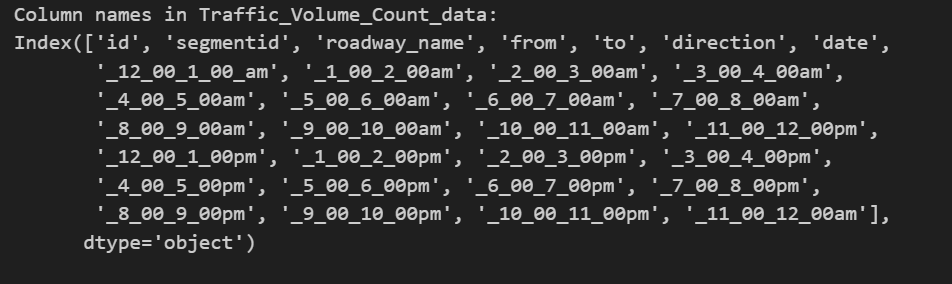
\includegraphics[width=1\linewidth]{figures/trafic_volume_count.PNG}
    \caption{Trafic Volume Count}
    \label{fig:Trafic Volume Count}
\end{figure}
\newline
\begin{figure}[h]
    \centering
    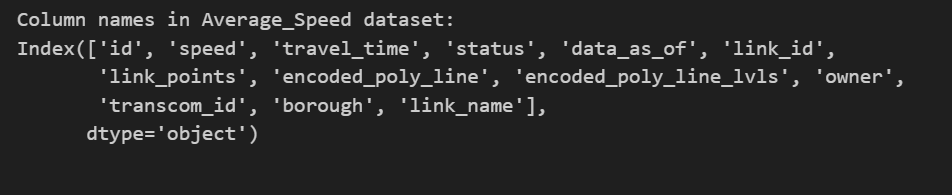
\includegraphics[width=1\linewidth]{figures/average_speed_dataset.PNG}
    \caption{Average Speed Of A Vehicle}
    \label{fig:Average Speed Of a Vehicle}
\end{figure}
\newline
We focused on optimizing traffic management for three road segments in New York City, defined as follows:
\newline
\newline
1. 5th Ave between 46th St and 47th St.\\
\begin{figure}[H]
    \centering
    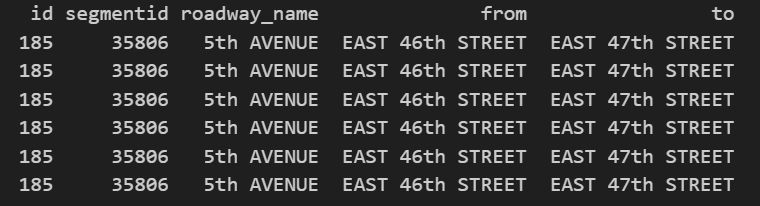
\includegraphics[width=\textwidth]{figures/area-1.PNG}
    \caption{First 5 columns from First Area}
    \label{fig:Data From Selected Area}
\end{figure}
2. Atlantic Ave between ALABAMA AVE and WILLIAMS AVE.\\
\begin{figure}[H]
    \centering
    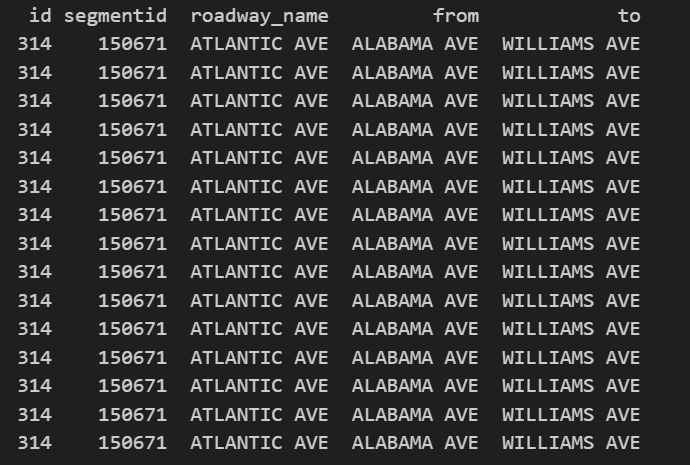
\includegraphics[width=\textwidth]{figures/area-2.PNG}
    \caption{First 5 columns from Second Area}
    \label{fig:Data From Selected Area}
\end{figure}
3. Queens Blvd between Union Tpke and Yellowstone Blvd (Queens).\\
\begin{figure}[H]
    \centering
    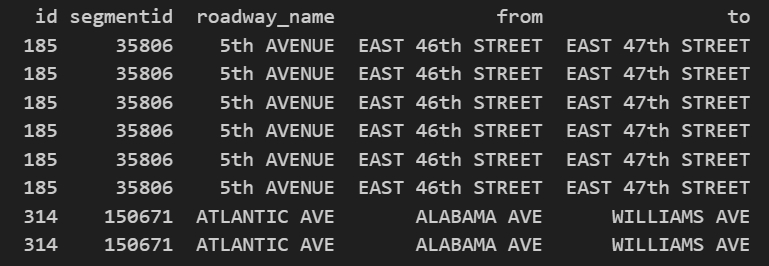
\includegraphics[width=\textwidth]{figures/area-3.PNG}
    \caption{First 5 columns from Third Area}
    \label{fig:Data From Selected Area}
\end{figure}
\begin{figure}[h]
    \centering
    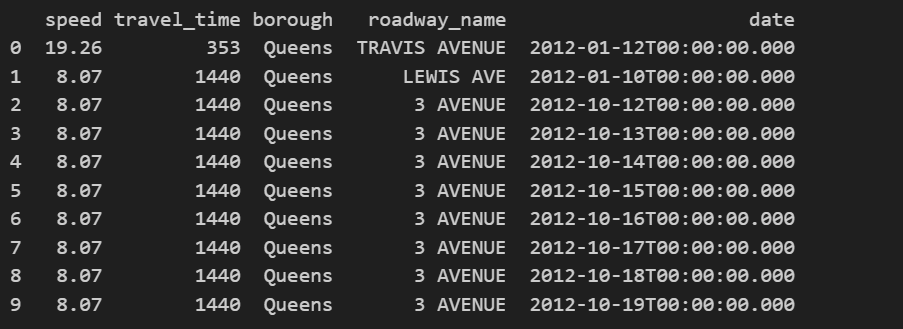
\includegraphics[width=1\linewidth]{figures/data_from_selected_area.PNG}
    \caption{Average Speeds From Selected Areas}
    \label{fig:Data From Selected Area}
\end{figure}
In order to use the data from the selected areas defined above, we merged all of them into one dataset, which was later combined with the Traffic Speed Data. Finally, we obtained a new dataset named Traffic Volume Count Data for Selected Area. 
\newline
This new dataset contains the sum of the columns from the two original datasets, which should total 31 + 13 = 44 columns. However, we ended up with an extra column due to the suffixing. 
\newline
We identified and preprocessed relevant data points, such as:
\newline 
\newline
\textbf{A. Peak-hour traffic volumes:}
\newline
\newline
 These were calculated based on the number of travel times during selected hours. To achieve this, we created a list of hourly columns in the New York City Data. The list is defined as follows:
\begin{figure}[H]
    \centering
    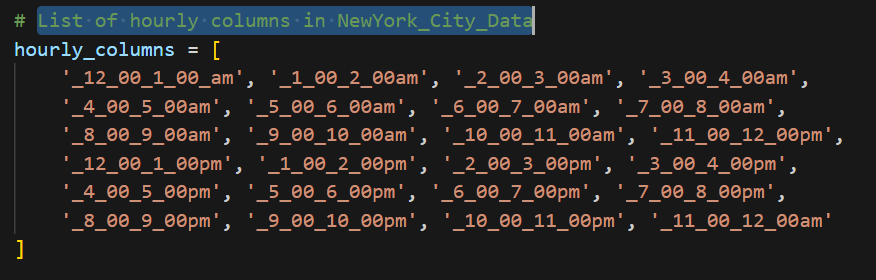
\includegraphics[width=\linewidth]{figures/List_of_hourly_columns.PNG}
    \caption{Traffic Volume Count Data for Selected Area}
    \label{fig:ListOfHourlyColumnsInNewYorkCity}
\end{figure}
To determine the overall peak hour, we first identified the peak hour across all records in the dataset. To calculate the peak hour based on the traffic data, we followed these steps[6]:
\newline
\begin{equation}
\text{Total Traffic Volume for Hour } h = \sum_{i=1}^{n} \text{Traffic Volume at hour } h_i
\end{equation}
where:
\begin{itemize}
    \item \( h_i \) represents the hour of each traffic record \( i \),
    \item \( n \) is the total number of records in the dataset for that hour.
\end{itemize}

\begin{equation}
\text{Peak Hour} = \arg \max_{h \in H} \left( \text{Total Traffic Volume for Hour } h \right)
\end{equation}
where:
\begin{itemize}
    \item \( H \) is the set of all possible hours in the dataset,
    \item \( \arg \max \) finds the hour that maximizes the total traffic volume.
\end{itemize}

\begin{equation}
\text{Maximum Traffic Volume} = \max_{h \in H} \left( \text{Total Traffic Volume for Hour } h \right)
\end{equation}
\newline
We calculated the total traffic for each hour and identified the maximum volume for each record across the dataset. As a result, the peak hour in New York City occurred from 7:00 to 8:00 PM, with an overall volume of 8,150,688 vehicles.
\begin{figure}[H]
    \centering
    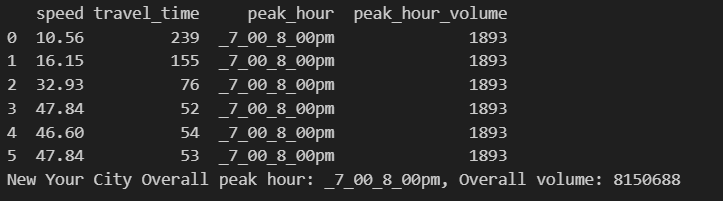
\includegraphics[width=1\linewidth]{figures/peak_huours.PNG}
    \caption{New York Peak Hours}
    \label{fig:New York Peak Hours}
\end{figure}

\textbf{B. Average speeds:}
\newline
The formula for calculating the average speed is given by[8]:
\begin{equation}
v_{\text{avg}} = \frac{\text{Total Distance}}{\text{Total Time}}
\end{equation}
For multiple vehicles, the average speed is:
\begin{equation}
v_{\text{avg}} = \frac{\sum_{i=1}^{n} d_i}{\sum_{i=1}^{n} t_i}
\end{equation}
Where:
\begin{itemize}
    \item \( d_i \) is the distance traveled by vehicle \( i \),
    \item \( t_i \) is the time taken by vehicle \( i \),
    \item \( n \) is the total number of vehicles or data points.
\end{itemize}
For hourly data, the average speed for a specific hour is calculated as:
\begin{equation}
v_{\text{avg\_hour}} = \frac{\sum_{i=1}^{n} v_i}{n}
\end{equation}
Where:
\newline
\begin{itemize}
    \item \( v_i \) is the recorded speed,
    \item \( n \) is the total number of measurements for that hour.
\end{itemize}
In order to calculate the average speed, we must first ensure that the speed data is in numeric format. The mean() function in Python allows us to compute the mean (or average) of a given set of values. As a result, we find that the average speed is 2513.80934 mph.
\begin{figure}[H]
    \centering
    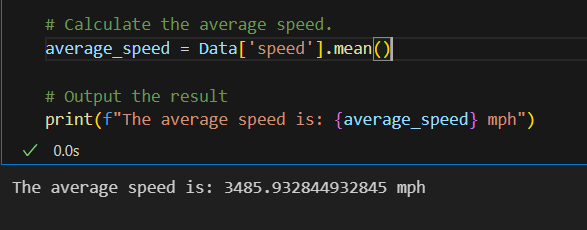
\includegraphics[width=1\linewidth]{figures/average_speed.PNG}
    \caption{New York Average Speed}
    \label{fig:new_york_peak_hours}
\end{figure}
\subsection{Fuel Consumption Calculation}
Fuel consumption measures the amount of fuel a car uses to travel a specific distance[4]. We used the standard fuel consumption equation, defined as follows:
\begin{equation}
\text{Fuel Consumption} = a \times V + b \times \frac{1}{V} + c
\end{equation}

Where:
\begin{itemize}
    \item \( V \) is the average speed (in mph),
    \item \( a \), \( b \), and \( c \) are empirical constants, with \( a \) indicating the increase in fuel consumption with speed, \( b \) representing a decrease in fuel consumption as speed increases, and \( c \) representing the base fuel consumption at very low-speed conditions.
\end{itemize}

The values of the coefficients \( a \), \( b \), and \( c \) are set as follows:

\begin{itemize}
    \item \( a = 0.01 \) is the coefficient for speed (\( V \)),
    \item \( b = 2 \) is the coefficient for \( \frac{1}{V} \),
    \item \( c = 0.1 \) is the constant term.
\end{itemize}

We then update the formula to calculate the total fuel consumption for each road segment and time interval by defining the following equation[10]:

\begin{equation}
\text{Fuel Consumption} = \sum_{i=1}^{n} \left( \text{Volume}_{i} \times \left( a \times V_{i} + b \times \frac{1}{V_i} + c \right) \times \text{Segment Length}_{i} \right)
\end{equation}

Where:
\begin{itemize}
    \item \( n \) is the number of time intervals,
    \item \( \text{Volume}_i \) is the vehicle count in interval \( i \) from the traffic volume dataset,
    \item \( V_i \) is the average speed in interval \( i \) from the traffic speed dataset,
    \item \( \text{Segment Length}_i \) is the length of the road segment.
\end{itemize}
However, in the selected area dataset, the peak hour volume refers to the vehicle count during the peak hour (Volume).
\newline
\newline speed is the average speed in mph.
\newline Segment represents the segment length in miles.
\newline
\newline
The following figure illustrates the data we have used.
\newline
\begin{figure}[h]
    \centering
    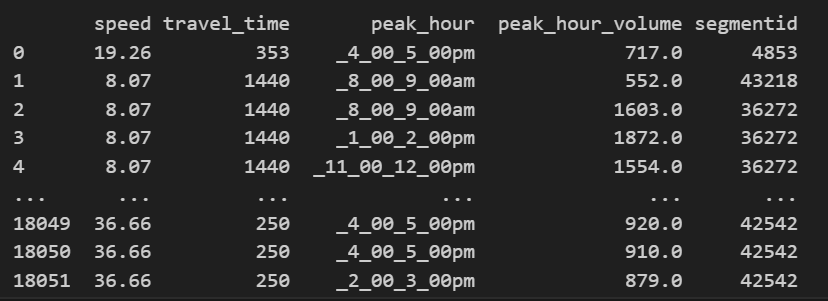
\includegraphics[width=0.7\textwidth]{figures/data_used_to_calculate_Total_Fuel_Consumption_For_each_road_segment.PNG}
    \caption{Selected Area Dataset}
    \label{fig:Selected Area Dataset}
\end{figure}
\newline
The following plot shows the fuel consumption for each time interval.
\newline
\begin{figure}[H]
    \centering
    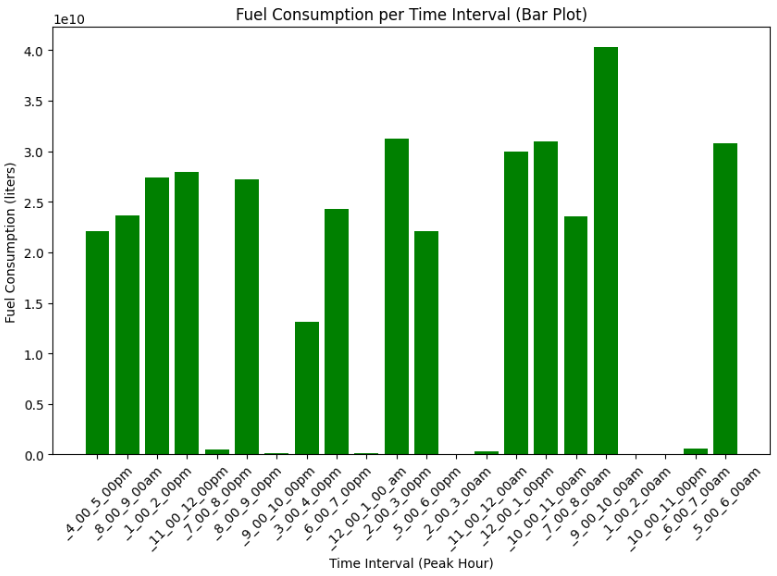
\includegraphics[width=1\linewidth]{figures/Fuel_consumption_per_time_interval.PNG}
    \caption{Fuel consumption per time interval}
    \label{fig:new_york_peak_hours}
\end{figure}
\subsection{Formulate the Optimization Problem}
We need the decision variables to represent the parameters that can be adjusted to optimize the traffic signal system and speed limits. These variables will be encoded in an individual in the genetic algorithm.
\newline
\newline A. Signal timings represent the durations of the green, yellow, and red phases for each intersection. This refers to the time allocated for each traffic signal phase—green, yellow, and red—at every intersection[11].
\newline 
\newline
B. Speed limit. They will be controlled in your optimization strategy.
The speed limit is a decision variable that defines the maximum speed allowed for vehicles on the road segment approaching each intersection[11]. 
\newline
\newline
We have defined the decision variables as follows:
\begin{itemize}
    \item \texttt{num\_intersections} = 3  \hspace{0.5cm} \# Number of intersections
    \item \texttt{max\_signal\_cycle\_time} = 120  \hspace{0.5cm} \# Maximum signal cycle time in seconds (sum of green, yellow, red)
    \item \texttt{speed\_limit\_min} = 30  \hspace{0.5cm} \# Minimum speed limit in km/h
    \item \texttt{speed\_limit\_max} = 120  \hspace{0.5cm} \# Maximum speed limit in km/h
    \item \texttt{green\_min} = 10  \hspace{0.5cm} \# Minimum green light duration in seconds
    \item \texttt{green\_max} = 60  \hspace{0.5cm} \# Maximum green light duration in seconds
    \item \texttt{yellow\_duration} = 3  \hspace{0.5cm} \# Yellow light duration in seconds
    \item \texttt{red\_min} = 10  \hspace{0.5cm} \# Minimum red light duration in seconds
    \item \texttt{red\_max} = 60  \hspace{0.5cm} \# Maximum red light duration in seconds
\end{itemize}
\textbf{A. Total Travel Time (TTT):} The total travel time is the time it takes for all vehicles to travel through the network of intersections during a given period. In the optimization, it works as follows[12]:

\begin{enumerate}
    \item \textbf{Green light duration:} The duration of the green light is very short, so vehicles will wait at the red light frequently.
    \item \textbf{Red light duration:} The longer the red light, the longer vehicles will wait.
    \item \textbf{Speed limits:} Higher speed limits generally result in faster travel times.
\end{enumerate}
\textbf{Objective Function for TTT:} The total travel time can be calculated as follows[12]:
\textbf{Total Travel Time (TTT):} The total travel time is the sum of the travel times for all vehicles through the network of intersections, considering both travel time and stop time. It can be expressed as[13]:

\[
\text{TTT} = \sum_{i=1}^{N} \left( \frac{d_i}{v_i} + T_{\text{stop}}(i) \right)
\]

Where:
\begin{itemize}
    \item \( N \) = Total number of vehicles in the network.
    \item \( d_i \) = Distance traveled by vehicle \( i \) (in meters or kilometers).
    \item \( v_i \) = Speed of vehicle \( i \) (in meters per second or kilometers per hour).
    \item \( T_{\text{stop}}(i) \) = Time spent stopping for red lights by vehicle \( i \) (in seconds).
\end{itemize}

\[
T_{\text{stop}}(i) = \sum_{j=1}^{M} \left( \text{Wait time at intersection } j \right)
\]

Where:
\begin{itemize}
    \item \( M \) = Number of intersections the vehicle passes through.
    \item The wait time.
\end{itemize}

Total travel time formula is:
\[
\text{Total Travel Time (TTT)} = \sum_{i=1}^{N} \left( \frac{d_i}{v_i} + \sum_{j=1}^{M} \text{Wait time at intersection } j \right)
\]
\begin{figure}[H]
    \centering
    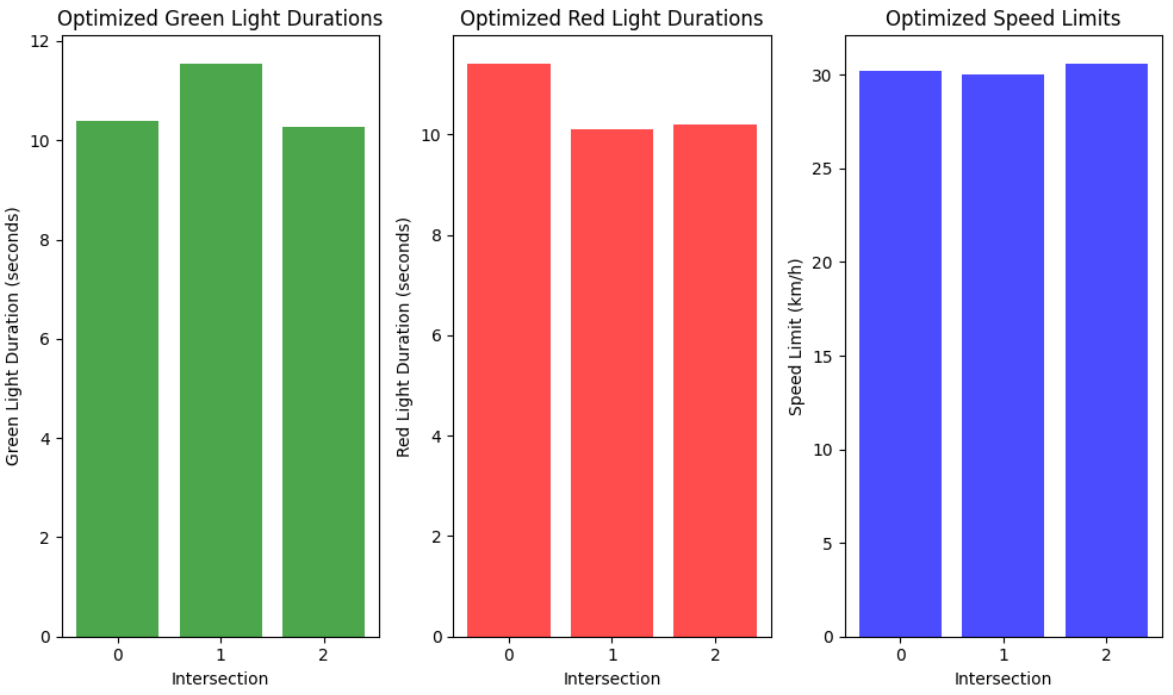
\includegraphics[width=1\linewidth]{figures/Optimizing_light_duration.PNG}
    \caption{Optimizing Red,Green, Yellow Light Duration}
    \label{fig:Optimizing Red,Green, Yellow Light Duration}
\end{figure}
\textbf{Fuel Consumption}: Is refers to the amount of fuel used by all vehicles in the network during a given time period. Optimizing fuel consumption is important for reducing environmental impact, improving air quality, and saving costs[12].
\newline
This system works to improve as follows:
\newline
1. Red light duration: Longer red light duration causes vehicles to stop for long periods, causing vehicle accumulation and congestion.
\newline
2. Speed limits: Lower speed limits can reduce fuel consumption by encouraging safer driving.
\newline
Fuel Consumption formula is:
\newline
\[
FC = \sum_{i=1}^{N} \left( \text{Red}_i \times C_{\text{red}} + \text{Speed}_i \times C_{\text{speed}} \right)
\]

Where:
\begin{itemize}
    \item \( N \) = Total number of vehicles or intersections
    \item \( \text{Red}_i \) = Duration of red light for vehicle \( i \) (in seconds)
    \item \( \text{Speed}_i \) = Speed limit for vehicle \( i \) (in km/h or m/s)
    \item \( C_{\text{red}} \) = Constant factor for red light fuel consumption (e.g., 0.1)
    \item \( C_{\text{speed}} \) = Constant factor for speed-related fuel consumption (e.g., 0.05)
\end{itemize}
\subsection{Implement the MOEA using Genetic Algorithm}
We designed an initial population of potential solutions (chromosomes) representing different traffic management strategies. To do this, we defined the structure of each individual (chromosome) and then initialized the population by randomly generating individuals within the specified constraints. Each individual consisted of three components: speed, green light duration, and red light duration.
\subsubsection{Initialization}
We started by implementing a genetic algorithm, initializing a population of individuals, where each individual represents a potential solution to the problem. Each individual is represented as a vector [speed, green light duration, red light duration], representing the vehicle speed and the traffic light durations. 
\newline
Chromosome Representation: Each individual is a 3-dimensional vector:
\newline A. The first element represents speed within the range [30, 120] km/h.
\newline B. The second element represents green light duration within the range [10, 60] seconds.
\newline C. The third element represents red light duration within the range [10, 60] seconds. However, population , and other decision variable has been initialized regarding our decision variable has been defined above.
\subsubsection{Objective Function}
The algorithm uses two objective functions, Total Travel Time (TTT), and Fuel Consumption (FC). These two objectives are calculated for each individual in the population, and the goal is to minimize both of them.
\subsubsection{Fitness Evaluation}
Each individual in the population is evaluated using the objective functions. Which they return tow dimintion valus, TTT, and FC.
\subsubsection{Selection}
 individuals are selected for reproduction (crossover and mutation) based on their fitness, with the goal of propagating the best traits to the next generation.
 \subsubsection{Crossover}
 it to introduces genetic diversity into the population and allows the algorithm to explore different combinations of variables.
 \subsubsection{Mutation}
 Each individual has a chance to mutate each of its variables (speed, green light, and red light duration).
 \subsubsection{Replacement}
 After the selection, crossover, and mutation steps, the offspring are added back to the population. The next generation of individuals is created by replacing the previous generation[14].
 \subsubsection{Termination and Pareto Front}
 The genetic algorithm iterates over a fixed number of generations defined in decition variable above. At each generation, the Pareto-optimal set of solutions is refined. the Pareto front is the set of individuals that represent trade-offs between the two objectives (TTT and FC)[14].
\begin{figure}[H]  % Exact placement
    \centering
    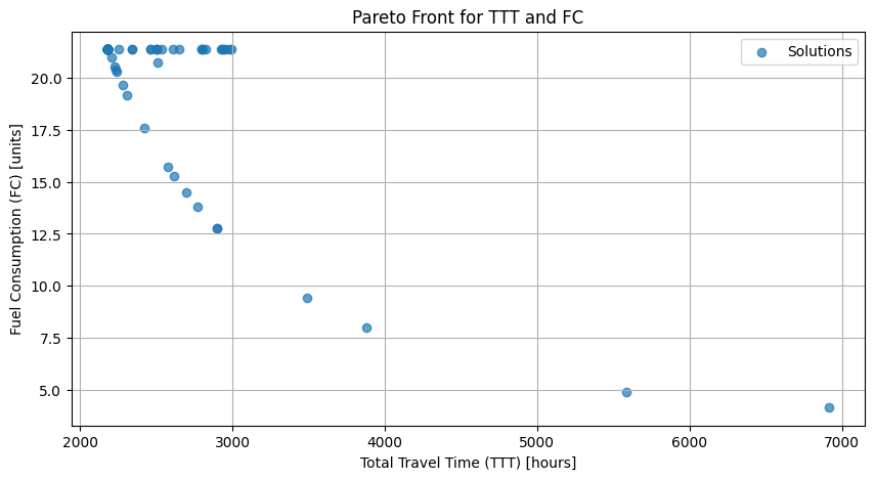
\includegraphics[width=\textwidth]{figures/TTT.PNG}
    \caption{Total Travel Time (TTT)}
    \label{fig:Total_Travel_Time}
\end{figure}

\clearpage  % Force next figure to be placed immediately
\begin{figure}[H]  % Exact placement
    \centering
    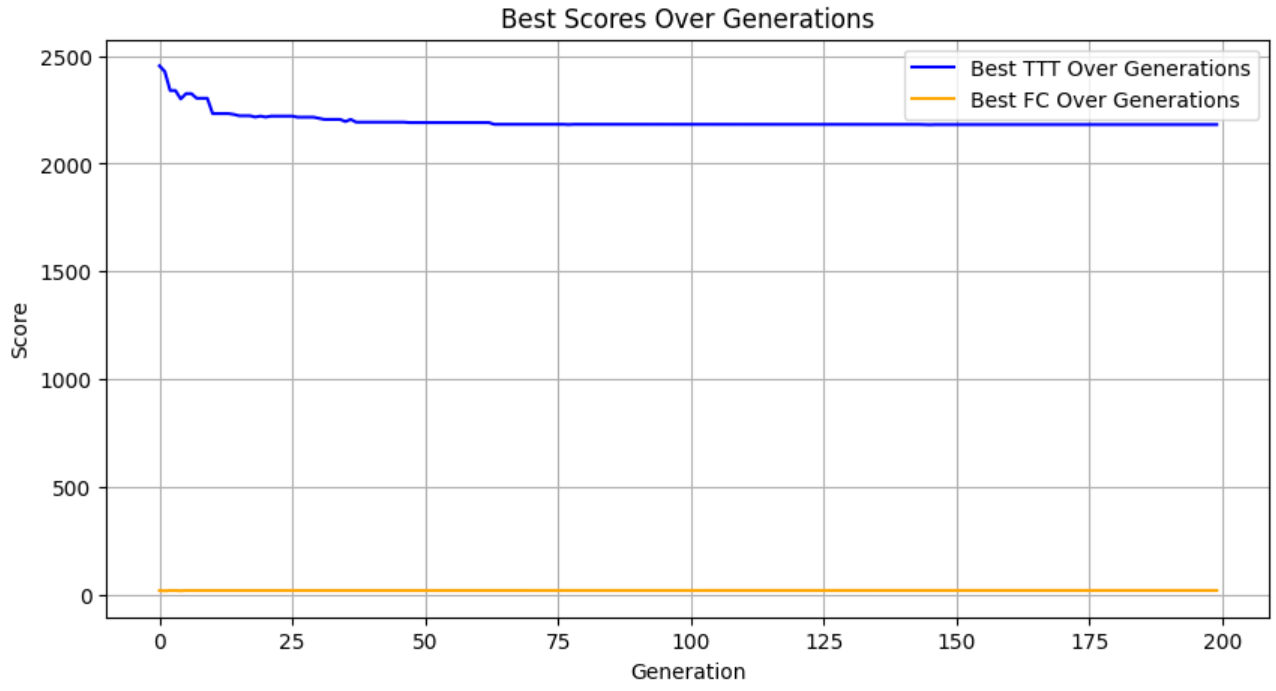
\includegraphics[width=\textwidth]{figures/Best_Score_Over_Generation.PNG}
    \caption{The Best Score Over Generations}
    \label{fig:Best_Score_Over_Generation}
\end{figure}










% Include the introduction
\section{Comparative Analysis of Evolutionary Programming and Evolutionary Strategies for Portfolio Optimization}
This assignment focuses on optimizing a financial portfolio with the single objective of 
maximizing expected return. You will implement and compare different versions of 
Evolutionary Programming (EP) and Evolutionary Strategies (ES) 
\subsection{Data Requirements}
sdjfksh

\includepdf[pages=-]{./Task_2.pdf}



% Include the results
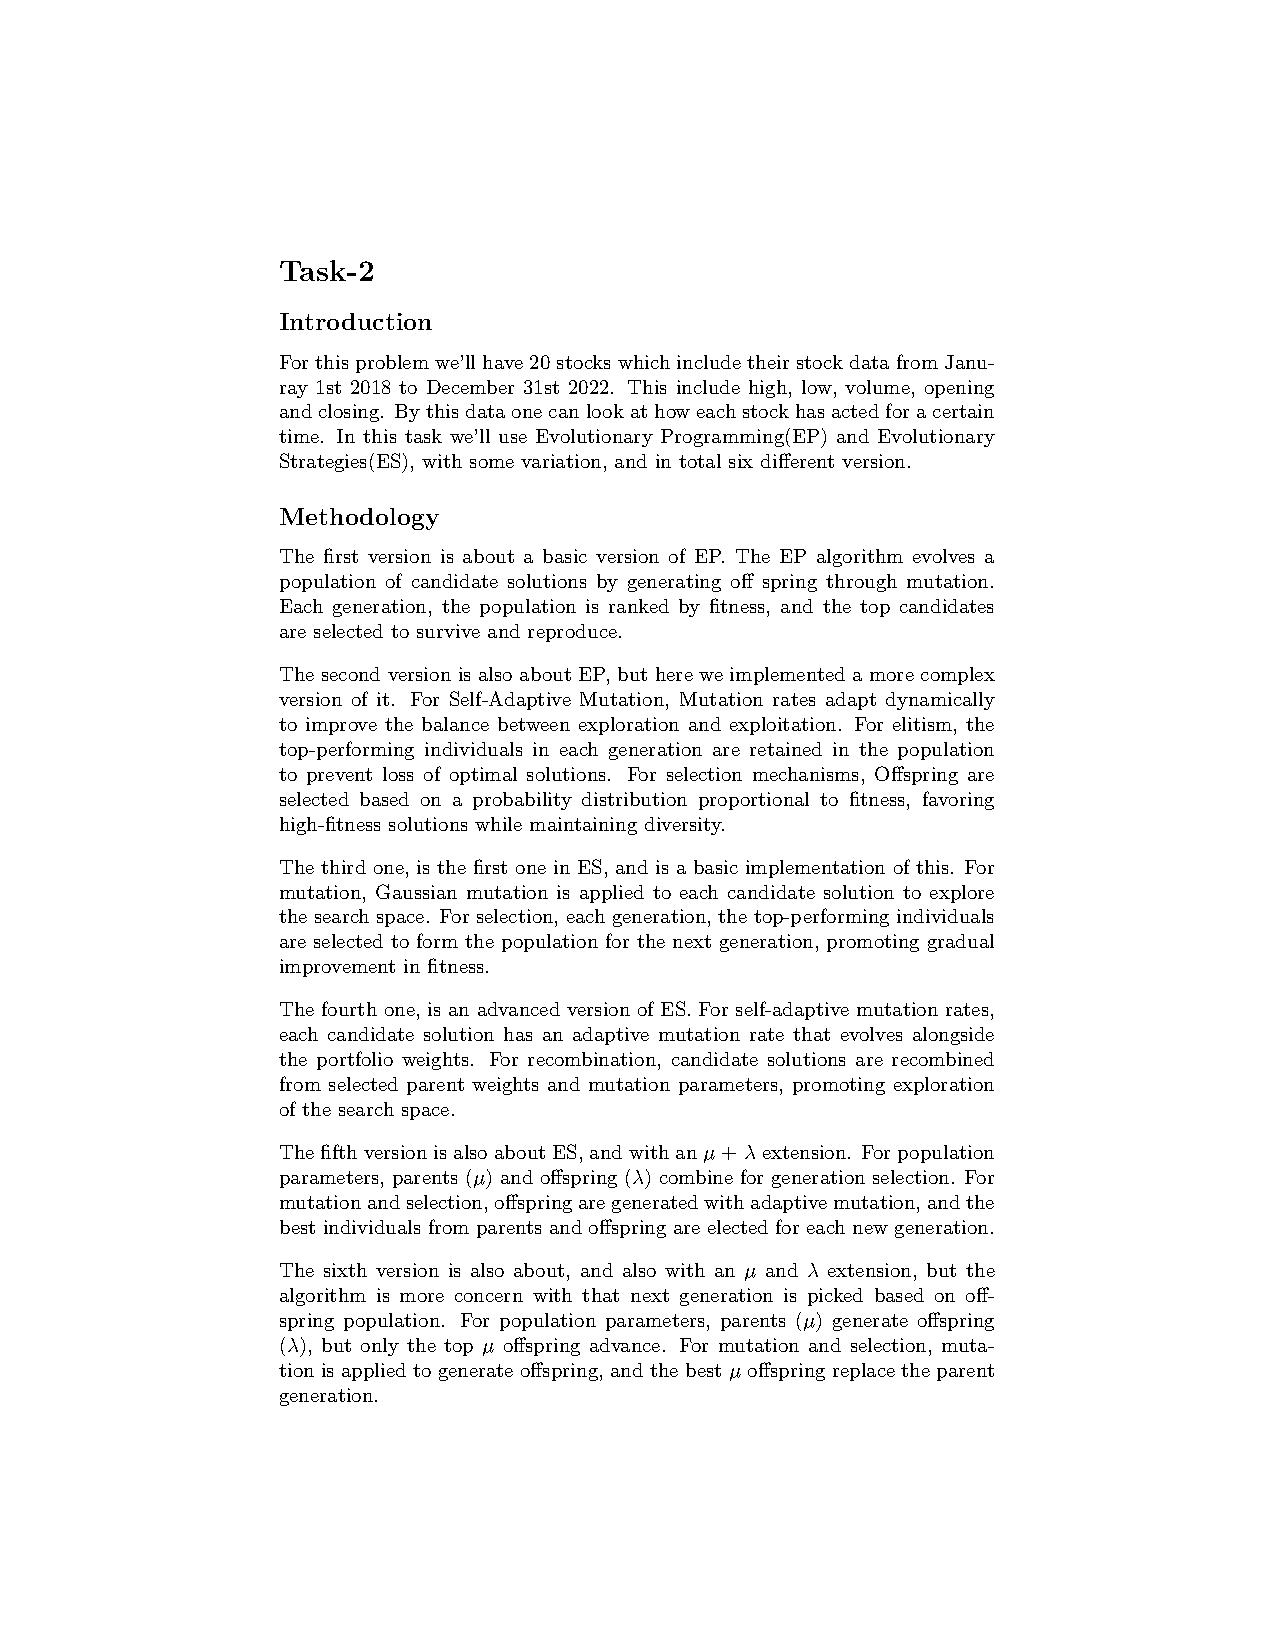
\includepdf[pages=-]{.\task_2.pdf}
% Include the results
\section{Task 4}
This is the introduction of the document. Here we will cite some references, for example, \cite{knuth1984texbook}.

% Include the results
\section{Refrences}
[1] NYC Open Data. "Traffic Volume Counts". 2022. Available at:
\newline
https://data.cityofnewyork.us/Transportation/Automated-Traffic-Volume-Counts/7ym2-wayt (Accessed: 2024-11-04).
\newline
[2] NYC Open Data. "DOT Traffic Speeds NBE". 2017. Available at: 
\newline
https://data.cityofnewyork.us/Transportation/DOT-Traffic-Speeds-NBE/i4gi-tjb9 (Accessed: 2024-11-04).
\newline
[3]Krivoshapov, S,  Nazarov, A ,  Mysiura, M , Marmut, I , Zuyev, V , Bezridnyi, V , Pavlenko, V. (2020). Calculation methods for determining of fuel consumption per hour by transport vehicles. IOP Conference Series: Materials Science and Engineering. 977. 012004. 10.1088/1757-899X/977/1/012004. 
\newline
[4] the official page of energy education. 
\newline
https://www.energyeducation.ca/encyclopedia/Fuelconsumption.


%\printbibliography

\end{document}
